\chapter{OpenCAL OpenCL version}\label{ch:opencal-cl}


This chapter introduces OpenCAL-CL, a porting of OpenCAL in OpenCL. OpenCL is a parallel framework originally proposed by Apple and then released as an Open Standard under the Khronos Group management. Besides computational efficiency, one of the main advantages of OpenCL is portability. In fact, you can run your program wherever you want across heterogeneous processors like Central Processing Units (CPUs), Graphics Processing Units (GPUs), Digital Signal Processors (DSPs), and Field-Programmable Gate Arrays (FPGAs).

OpenCAL-CL inherits many OpenCAL's features, by also adding parallel computation capability thanks to the adoption of OpenCL. The application is now subdivided in two parts: the \emph{host program}, running on the CPU, and the \emph{device program}, running on a compliant computational device (e.g. an Nvidia or AMD GPU). The CA object is still defined host-side, as in OpenCAL, while elementary processes (and possibly other functions) are defined device-side. Belonging to the device program, elementary processes must be defined as OpenCL's \emph{kernels} and therefore the programmer has to be able to write some minimal OpenCL code to implement them. Fortunately, OpenCAL-CL hides lots of parallel aspects to the user (e.g. the simulation loop is internally managed by the library) and also simplifies data exchange between host and device. The users's OpenCL parallel programming background can be therefore limited or even null. In the latter case, the user can learn some basic elements of OpenCL kernel programming thanks to this guide.

This chapter is divided into two parts: the first part is a very brief overview of OpenCL, while the second one introduces OpenCAL-CL by examples.

\section{OpenCL framework}
OpenCL enables parallel programming that assigns computational tasks to multiple processing elements to be performed at the same time. These tasks are called \emph{kernels}. The kernel is a special function that can be executed to different OpenCL-compliant devices. In the OpenCAL library, each elementary process of the CA transition function can be devised as a kernel.
The kernels are sent to the device(s) by the host application. The host application defines a structure called \emph{context}, needed to manage data exchange and computation on the compliant devices.

In particular, host application links kernels into one or more programs In the host application, the user can select the kernel's functions to insert inside a container called \emph{program}.  The program connects the kernel with argument data and dispatches it to a structure called command queue.  The command queue is a structure that allows the host to decide what the devices have to do, and when a kernel is enqueued, the device will execute the relative function.

\begin{figure}[htp]
  \begin{center}
    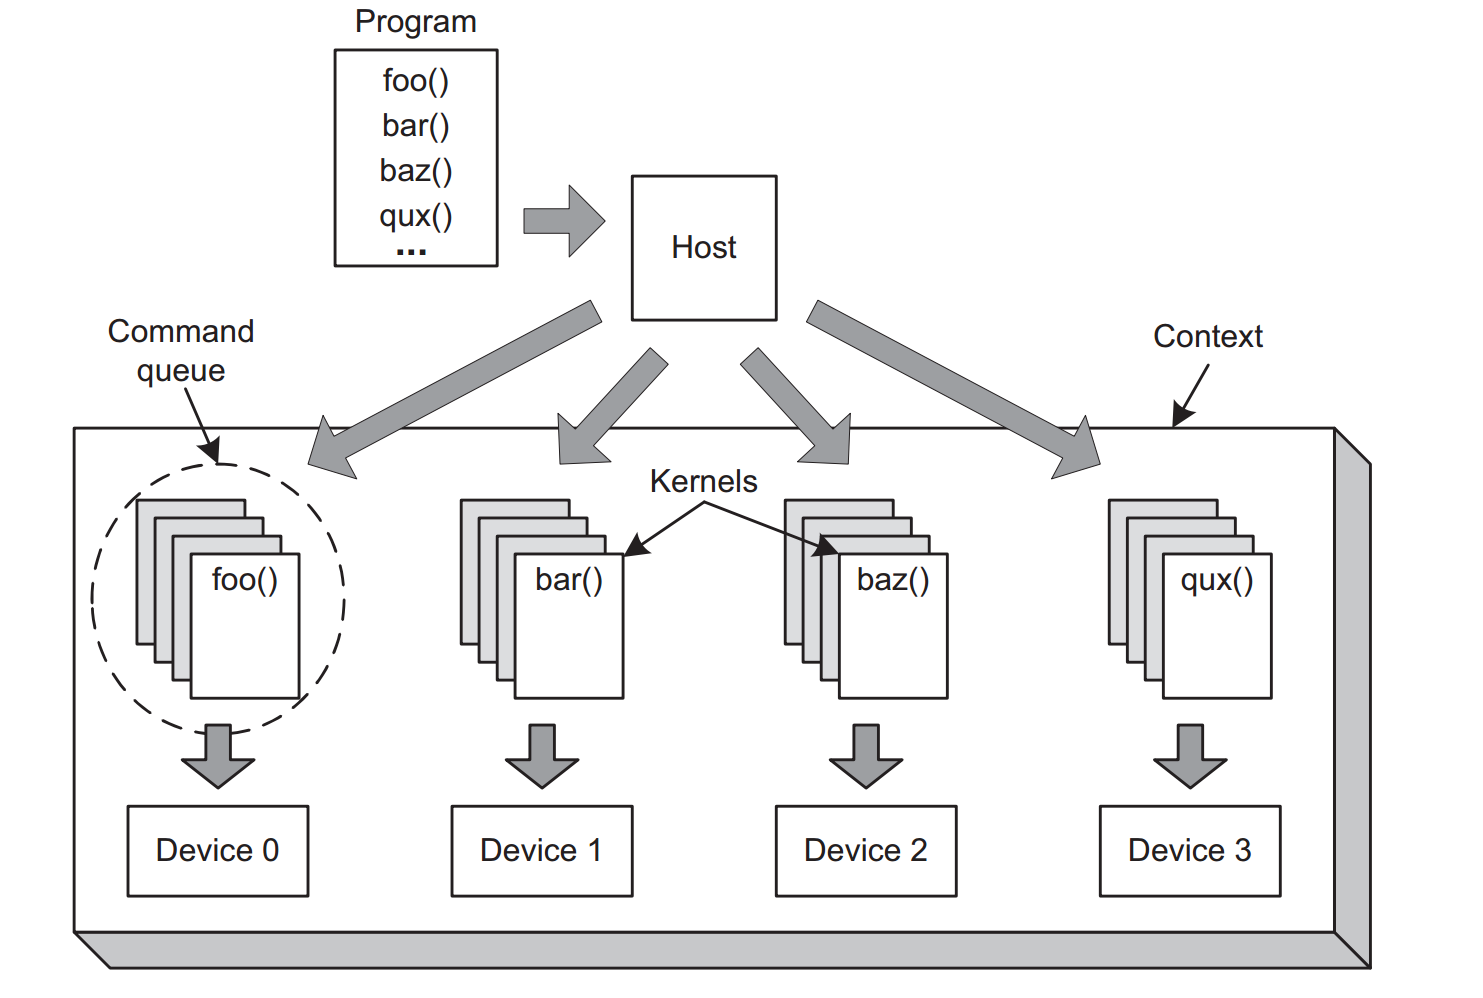
\includegraphics[width=12cm]{./images/OpenCAL-CL/kernelDistribution}
    \caption{General structure of a OpenCL program}
    \label{fig:GeneralStructure}
  \end{center}
\end{figure}

As we can see from the picture above, the context contains all the devices, all the command queues and all the kernels.
More in detail, for every device a command queue is associated and every command queue has inside all the kernel functions
that the device has to execute.

\section{The structure of OpenCAL-CL}
As each OpenCL applications, the library OpenCAL-CL has a set of structures and
functions to develop host program and to define kernels. The definition of the
CA is specified in the host program. The user can define two types of models, 2D or
3D, as shown in \ref{ch:opencal}. 
The host program manages the kernels and dispatches the data of the model, like substates, the type of neighbourhood, 
size of the cellular space, etc, to the computation units.
The host program
manages the execution loop and which computation unit has to execute the
transition functions. \\
The host program is typically divided in the following sections:
\begin{itemize}
\item definition of the model (Chapter \ref{ch:opencal}) 
\item management of the OpenCL devices
\item kernels allocation
\item data sending from the model to devices
\item execution loop start
\end{itemize}

\section{Host programming} 

\subsection{Definition of the model}

XXX

\subsection{Manage of the devices}

After the model creation, the user must choose the device for the kernel computation.
Inside the library a structure called CALOpenCL allows the user to manage all 
available platforms and devices.
This structure simplifies the access to the devices compared with the native API
of OpenCL. The library supplies other functions to know which platforms and
devices are available on the system and to have information about these.\\
Below you can see a simply program that explains how the 
CALOpenCL structure can be used.


\begin{lstlisting}
#include <calCL2D .h>

 int main (){

 CALOpenCL * calOpenCL = calclCreateCALOpenCL ();
 // get all available platforms
 calclInitializePlatforms ( calOpenCL );
 // get all available devices
 calclInitializeDevices ( calOpenCL );

 // get the first device on the first platform
 CALCLdevice device = calclGetDevice ( calOpenCL , 0, 0);

 // create a context
 CALCLcontext context = calclcreateContext (& device , 1);

 return 0;
 }
\end{lstlisting}

Inside the library, the platforms and the devices are store in a matrix where rows represent the platforms and columns represent the devices. Thus, to choose which one we can use for the computation,
it's necessary to specify the index of platform and the index of the device. For
example, at lines 12, we chose the platform number
0 and the device number 0. If we have a system with 3 NVIDIA GPUs and 3 AMD GPUs, the library will have a 2x3 size matrix, where 2 are the vendors (i.e, the platforms NVIDIA and AMD) and 3 are the GPUs for each platforms. If we want to 	
run the program to the third AMD GPU we can specify as indices 1 and 2.
If we don't know how the system identify the platforms and devices, the
library give us a function called \verb'calclGetPlatformsAndDeviceFromStandardInput'
the allows us to know the platforms and device. First it prints the
information on standard output and then we can insert the indexes directly from
standard input.\\
After we chose the device, the user must specify the path where are the kernels
and relative headers.
Through the function \verb'calclLoadProgramLib(2D/3D)' the library reads automatically
the kernels and compiles their.
\begin{lstlisting}
CALCLprogram calclLoadProgramLib(2D|3D) ( CALCLcontext context ,
CALCLdevice device , char * path_user_kernel , char *
path_user_include )
\end{lstlisting}

\subsection{Allocation of kernels}

The library doesn't know which kernels (i.e., the CA elementary processes) they have to run, for this reason the
user must specify the names of the kernels.
To create and allocate a kernel it's necessary to call the function
\verb'calclGetKernelFromProgram' that gets an OpenCL kernel given a compiled OpenCL
program. 

\begin{lstlisting}
cl_kernel elementaryProcess = calclGetKernelFromProgram(&program,
KERNEL_NAME);
\end{lstlisting}


\subsection{Send data from the model to devices}

To transfer the data from host side to kernel side, the user must define the
 structure called \verb'CALCLToolkit(2D/3D)' containing all the buffers (data) of the
model.
By default the library sends to all the kernels the data belongs to the model. The following list shows the
data sended:
\begin{itemize}
	\item the dimension of cellular space 
	\item the number of substate for every type (byte,int,real) 
	\item the substates allocated from the user
	\item the list of active cells
	\item the list of active cells flags
	\item type, dimension and ID of the neighbourhood
	\item the border condition
\end{itemize}


 First the user must create an
instance of the structure \verb'CALCLToolkit(2D/3D)' through calling the function
\verb'calclCreateToolkit' as shown the following code
\begin{lstlisting}
CALCLToolkit2D * calclCreateToolkit (2D|3D)(struct CALModel (2D|3D) *model ,CALCLcontext context ,CALCLprogram
program ,CALCLdevice device ,CALCLOptimization opt)
\end{lstlisting}
The enumerative \verb'CALCLOptimization' allows the user to choose if it wants to use
the library without optimization \verb|(CALCL_NO_OPT)| or with active cells optimization
 \verb|(CALCL_OPT_ACTIVE_CELLS)|. The structure \verb'CALCLToolkit(2D/3D)'
doesn't contain only the buffers to transfer data but also the kernels belong to the
excution loop. \\
To add a new kernel to the execution loop the user have to call the function \verb'calclAddElementaryProcessKernel(2D/3D)' that
adds the chosen kernel to the list of elementary processes moreover it sends to
the device all the necessary data to execute the kernel.

\begin{lstlisting}
void calclAddElementaryProcessKernel2D(CALCLToolkit2D * toolkit2d, struct CALModel2D *model, CALCLkernel * elemProcKernel);
\end{lstlisting}


\subsection{Start execution loop}

To start the execution loop the user have to call the function \verb'calclRun(2D/3D)'. The function executes
all the elementary processes previously declared on the specified device.

\begin{lstlisting}
void calclRun2D(CALCLToolkit2D* toolkit2d, struct CALModel2D * model, unsigned int initialStep,	unsigned maxStep);
\end{lstlisting}


\section{Kernel programming} 

In order to use OpenCAL, you need to include some header files.
Specifically, cal2D.h or cal3D.h allows you to use some simply 
functions to interact with the data structures belong to the model.
To create a kernel function in OpenCL we must use 
the key word \verb'__kernel' before the returing 
type of the function. In OpenCAL-CL every time 
we create a kernel function you must specify as first parameter
 the key word  \verb'MODEL_DEFINITION2D' and call the function \verb'initThreads2D()' as first 
 istruction.\\
The code below shows how to declare a new kernel.
\begin{lstlisting} 
__kernel void kernel(MODEL_DEFINITION2D){
					initThreads2D();
					...
					...
					...
}
\end{lstlisting}

When the user is going to implement an elementary process, by defining its
kernel function, he/she can rely on a set of OpenCAL functions that allow to
get the substates values of both the central and the neighbouring cells, and to
update the substates values of the central cell. Every time the user wants to use 
this function he/she must pass as first parameter the key word  \verb'MODEL2D'. 
For example if we want to get the value of a specific cell we need to use 
the function \verb'calGet2Dr'.
\begin{lstlisting} 
	double a = calGet2Dr(MODEL2D, 0, i, j);
\end{lstlisting}
The function get the value of the cell i, j of the substate 0.\\
Given that, inside OpenCAL-CL you can use all the OpenCL features,
you can exploit all the memory level as global memory, local memory, 
private memory (citazione libro). In order to use these memory level, 
we must declare the variables using this specific syntax respectively \verb'__global', 
\verb'__local', \verb'__private'.

\subsection{Conway’s Game of Life}

As we did in \ref{sec:cal_life}, in order to introduce you to Cellular Automata 
development with OpenCAL-CL, we start implementing the Conway’s Game of Life.
Below you can see the host program of the Conway’s Game of Life:
\lstinputlisting[label=lst:cal_sciddicaT, caption=An OpenCAL-CL implementation of the Conway's game of Life.]{../opencal/OpenCAL-CL/examples/calcl_life/source/life.c}
code descriptions \\
Here you can see the device code of the Conway’s Game of Life:
\lstinputlisting[label=lst:cal_sciddicaT, caption=An OpenCAL-CL kernel to implement the Conway's game of Life elementary process.]{../opencal/OpenCAL-CL/examples/calcl_life/kernel/source/life.cl}




  
